% ==============================================================================
%
% "Ideas for Citizen Science in Astronomy"
%
% Marshall, Fletcher, & Lintott, ARAA (2014)
%
% ==============================================================================

\documentclass{ar2e}

\usepackage{ulem}
\usepackage{ARAstroBib}
\usepackage{amssymb,amsbsy,psfig}
\usepackage{xspace}
\usepackage[usenames]{color}
\usepackage{graphicx}

% JOURNALS
\def\apj{ApJ}                                         
\def\apjs{ApJS}
\def\apjl{ApJL}
\def\aap{A{\&}A}
\def\aaps{A{\&}AS}
\def\mnras{MNRAS}
\def\aj{AJ}
\def\araa{ARAA}
\def\pasp{PASP}
\def\nat{Nature}
\def\prd{Phys.\ Rev.\ D}

% MISC
\def\eg{{\it e.g.}\xspace}
\def\ie{{\it i.e.}\xspace}
\def\cf{{\it c.f.}\xspace}
\def\etal{et~al.\xspace}

% CROSS-REFERENCES
\def\Sref#1{Section~\ref{#1}\xspace}
\def\Fref#1{Figure~\ref{#1}\xspace}
\def\Tref#1{Table~\ref{#1}\xspace}
\def\Eref#1{Equation~\ref{#1}\xspace}
\def\Eqref#1{Eq.~(\ref{#1})\xspace}

% COMMENTING
\newcommand{\phil}[1]{\textcolor{blue}{\bf PJM: #1}}
\newcommand{\chris}[1]{\textcolor{blue}{\bf CJL: #1}}
\newcommand{\leigh}[1]{\textcolor{blue}{\bf LDF: #1}}
\newcommand{\todo}[2]{{\bf \it TODO: #1: #2}}
\newcommand{\query}[2]{{\it \textcolor{red}{Q: #1: #2}}}
\newcommand{\answer}[2]{{\it \textcolor{blue}{A: #1: #2}}}


% ==============================================================================

\begin{document}

% ------------------------------------------------------------------------------

\jname{Annu.\ Rev.\ Astron.\ Astrophys.}
\jyear{2014}
\jvol{}
\ARinfo{}

\title{Ideas for Citizen Science in Astronomy}

\author{Phil Marshall,$^{1,2}$
Leigh Fletcher,$^{2}$ and
Chris Lintott$^{2}$
\affiliation{%
\small
$^1$ Kavli Institute for Particle Astrophysics and Cosmology, P.O.~Box~20450, \newline
MS~29, Stanford, CA 94309, USA. \newline
$^2$ Department of Physics, Denys Wilkinson Building, University of Oxford, \newline
Keble Road, Oxford, OX1 3RH, UK.}}

\markboth{Marshall, Lintott \& Fletcher}{Citizen Science in Astronomy}

% ------------------------------------------------------------------------------

% \begin{keywords}
% Go here...
% \end{keywords}

\begin{abstract} 

We review the relatively new, internet-enabled, and rapidly evolving field of
citizen science, focusing on ideas from which astronomy either has benefited, or
could benefit in the future. We consider contributions to science in the form of
observations, instrumentation, data processing, data modeling and the design of
new scientific inquiries. Engaging a large and diverse community of both
professionals and citizens, we digest and present their suggestions for ideas
for citizen astronomy in the future. The limits to this approach to scientific
investigation are not yet known, but we make some rough estimates for astronomy
in particular.

\end{abstract}

\maketitle

% ==============================================================================

\section{Introduction (2 pages)}
\label{sec:intro}

The term ``Citizen Science'' refers to the activities of people who are not paid
to carry out scientific research, but nevertheless make intellectual
contributions to scientific research in their spare time. These contributions
are diverse, both in type and research area. The people who make those
contributions can, and do, come from all walks of life. This review is about the
science projects they have participated in to date, the tasks they have
performed, and how astronomy has benefited -- and could benefit further -- from
their efforts.

Citizen involvement in science pre-dates the profession itself, and there is a
long and honourable tradition of amateur observers making important discoveries
and significant sustained contributions. However, the advent of the world wide
web has changed the face of professional and amateur collaboration, providing
new opportunities and accelerating the sharing of information. People are now
connected to each other in a way that has never happened before. Professional
scientists can interact with citizens via a range of web-based media, including
purpose-built citizen science websites which increase the potential for shared
data analysis and exploration as well as data collection. Meanwhile, communities
of citizens have sprung into existence as like-minded people have been able to
find and talk to each other in a way that is almost independent of their
geographical location. The result has been an exponential increase in citizen
involvement in science. The field is evolving very quickly, with more and more
professional scientists becoming aware of the possibilities offered by
collaborating with, for example, specialists operating outside the usual
parameters of professional astronomical observation, or tens of thousands of
people eager to perform analysis in their lunch hours via microtasking.  Our aim
in this review is to review the scientific literature as it stands for ideas
implemented in citizen science projects, primarily in astronomy but also in
other fields, and then produce a summary of successful project characteristics
for future research groups to learn from.

As our title states, this is a review of ideas for astronomy. We will look
forward as well as back, and try to answer the questions: How can the full
potential of citizen science be realised in astronomy? What are the particular
niches that citizen science can fill, in our field? How might it contribute to
the solutions of the Big Data problem in astronomy?

% Somewhat in the spirit of citizen science, we are crowd-sourcing these
% questions via a blog, \stellarpops, set up to accompany this article.  Each
% area we cover will be opened up for discussion in the comments section, and we
% are encouraging the leading proponents to join in that discussion. Likewise,
% we are encouraging involvement from the citizens already working in astronomy,
% and the  community of astronomers collaborating with them. The result will be
% an open conversation which we will distill, with appropriate acknowledgment,
% into these pages.
% 
% \BLOG{1}{Phil}{What's all this about?}

This review is organised as follows. We survey the contributions to science that
citizens have made to date, organized according to the stage of the scientific
enquiry that those contributions fell into. Astronomy research typically starts
with observations: so do we, in \Sref{sec:obs}. We then proceed through a
discussion of citizen instrumentation, data processing, data modeling and
finally citizen-led enquiry in 
Sections~\ref{sec:instr}--\ref{sec:explore}. With this overview in place,
we review in \Sref{sec:crowd} the literature on, and the collected experience
of, the population of citizens who have taken part, or are currently taking
part, in scientific research, before summarizing progress in citizen science to
date in \Sref{sec:summary}. In the second part of this review, we turn to the
future. We first report a variety of suggestions for how
citizens might contribute to astronomy there in \Sref{sec:future}. Then, in 
\Sref{sec:limits} we consider possible limits to citizen science, including
challenges associated with data rates and volumes, data complexity, the
difficulties of large-scale collaboration, and finally the barriers to
accessibility. Finally, we give some concluding remarks in
\Sref{sec:conclusions}.


% ------------------------------------------------------------------------------

\section{Data Acquisition: Citizen Observing (5 pages)}
\label{sec:obs}

Typically, data in astronomy is aquired with some sort of telescope. In the 21st
century there certainly is an active community of well-equipped amateur
observers making observations of great utility. There are also many other
citizens observing the night sky with less sophisticated equipement, and/or less
enthusiasm -- and as we shall see, there are plenty of citizens making 
astronomical observations almost inadvertently. What astronomical data are the
citizenry taking, and what is it being used for?

% - - - - - - - - - - - - - - - - - - - - - - - - - - - - - - - - - - - - - - - 

\subsection{Active Observing (\textbf{Leigh}, Chris to edit, 3 pages)}
\label{sec:obs:active}

The steady improvements and increasing affordability of digital technology, in
addition to the ease of data sharing and communications, have considerably
expanded the realm of amateur astronomy in the past two decades.  Observers
have always been passionate about their pastime, from painstakingly recorded
hand drawings of the planets and their positions in the night sky, to hours
devoted to the monitoring and tracking of astronomical events.  There is a
long and proud history of contributions from ?amateurs? to the field, driven
by a desire to share the results of their hobby with others.  But it has only
been in the past few decades that regular and systematic pipelines have been
in place to share data between amateurs and professionals, enticing passionate
observers to shape their observations to address scientific questions.  In
this section, we review some of the citizen contributions to active
observations of the night sky.  Passive contributions, via data mining and
web-based studies, will be described in Section \ref{}.

Why is active citizen observing beneficial to professional astronomers?  The
key advantage is time ? the very core of astronomy is observational, and
intense competition for resources means that professional astronomers are
unable to continuously monitor all the objects of interest in the night sky. 
Indeed, professional observatories are always oversubscribed, with resources
concentrated on one area of sky, or one astronomical question.  Observations
from professional telescopes, space-based observatories and visiting planetary
missions are often sparse and poorly sampled due to extreme competition for
resources.  Such observations are rarely tuned to the optimum timescales for
scientific enquiry ? for example, determinations of meteor frequencies on
short timescales (minutes), or slow evolution of giant planets on longer
timescales (years and decades).  Amateur observations can be frequent and
repetitive to provide monitoring of astronomical targets, and are naturally
well sampled across the globe during an exciting event of interest. 

The second, related, advantage is that of flexibility ? whenever a new
phenomenon is discovered (e.g., a new comet, or anything changing the
appearance of the familiar planetary discs), observers will be keen to catch a
glimpse irrespective of the scientific value of their observations.  This
reaction can be near instantaneous, compared to the need to allocate telescope
resources among the professional community.  The third benefit is contextual ?
global maps of an object's visible albedo provide useful additional
constraints on a process of interest, especially when near-simultaneous
professional observations occur in a vastly different wavelength range (e.g.,
UV or infrared); over a narrow spatial region (e.g., close-in studies by
spacecraft); or employ spectroscopic techniques that don?t yield images. 
Comparisons with the visible albedo provided by citizen scientists can
therefore play an extremely useful role in planetary missions, both for
context and for observation planning.  Active observation by enthusiastic
citizens contributing directly to scientific progress, combined with the
excellent communication channels that have opened up in the past two decades,
and the digital technology that allows astrophotographers to shine, is
beginning to plug this observational gap.

As a result of these benefits, a few professionals are very closely linked
with the amateur community, organising publications and assisting in
observation planning to maximise science return.  New planetary missions
frequently involve scientists to serve as an interface with the amateur
community (this is particularly true to the 2016-17 Juno mission to Jupiter). 
In return, amateurs trigger alerts through online forums or emails to
professional networks, announcing a tentative new discovery to the world for
scrutiny and follow-up. The benefits of strong professional-amateur
collaboration will be repeated in the following examples where active
observations have contributed directly to our understanding of our place in
the universe.  We do not intend a complete review of all examples of Pro-Am
collaboration, but a few representative examples.  For a detailed review of
the methodology employed by amateur observers, the reader is referred to
\citet{13mousis}.  Within our solar system, active observations fall into two
interconnected categories:  Discovery and Monitoring, where each will almost
certainly lead to the other.
 
\subsubsection{Discovery-Class Science}

Discovery-class citizen science is enabled by the quantity of data obtained
and the extreme familiarity of citizen astronomers with a particular region,
planet or nebula, allowing them to immediately identify peculiarities or new
features \citep[e.g., meteorological activity on giant planets,][]{95rogers}. 
Solar system objects moving against the fixed-star background can be detected
in a set of CCD frames either by eye or by automated software.  The position
of this new object is then compared to existing catalogues, and if no existing
details are found then the new discovery and its ephemerides can be reported
to the IAU Minor Planet Centre\footnote{http://www.minorplanetcenter.net}.  If
observations are repeated for at least two nights by one or several observers,
then a new denomination is provisionally assigned to the discovery.   An
electronic circular then reports the discovery to the wider world.  Suitable
targets for these searches include near-earth asteroids (NEAs, with orbits
intersecting those of the terrestrial planets), main belt asteroids between
Mars and Jupiter, and comets making their journey towards the Sun from the
outer solar system.  

The recent close flyby of asteroid 2012 DA14 on February 15th 2013 was
initially reported by a team of amateur observers affiliated with the La Sagra
Sky Survey at the Astronomical Observatory of Mallorca.  Amateur observers
still contribute to the discovery and photometric imaging of comets, and many
amateurs have managed to become associated with new cometary discoveries,
including David Levy, part of the team that discovered Shoemaker-Levy 9 before
its spectacular impact with Jupiter.  As with asteroids, the majority of new
comet discoveries are made by automated surveys, but a small and stable number
of discoveries come from amateurs with small telescopes, typically in regions
poorly covered by survey telescopes (e.g., regions close to the Sun).  C/2011
W3 Lovejoy, a Kreutz sungrazer comet, is one such example.  C/2012 S1 ISON was
spotted by A. Novichonok and V. Gerke in images from the International
Scientific Optical Network.  One might imagine that, as observing technology
improves, citizen discoveries via active observation might extend out to the
distant Kuiper Belt, although many of these targets are so dim that they are
unavailable to all but the largest of apertures.

Although survey telescopes provide the vast majority of modern discoveries,
citizen observations allow detailed characterisation of physical and orbital
characteristics of these newly discovered solar system bodies, and amateur-led
contributions are published
online\footnote{http://www.minorplanet.info/mpbdownloads.html}.  There is a
need to continuously track Near Earth Asteroids as gravitational effects can
significantly alter orbital trajectories over time, and this astrometry for
both asteroids and comets can be provided to the Minor Planet Centre for
collation and use in computing orbital trajectories.  Amateur monitoring of a
comet?s coma, dust and plasma tails and their photometric parameters can
reveal dynamic structures and determine the locations of active venting
regions.  Photometric monitoring of comets over time of the magnitude and tail
characteristics provides insights into the levels of activity as the comet
moves along its trajectory, and can also reveal outbursts and other events
associated with the outgassing.  Photometric monitoring of an asteroid as it
rotates provides information on the physical parameters, such as the shape,
rotation rate and orientation.  Observationas of mutual encounters can also
yield information on the density, and hence the composition of the asteroids.

Amateurs are also contributing to the search for a sub-category of objects
with a detectable cometary coma within the asteroid belt.  Recent discoveries
of these Main Belt Comets, which appear to be asteroids that are actively
venting their volatiles at perihelion, are beginning to blur the distinction
between asteroids and comets.  The T3 project, a collaboration between the
University of Rome and several amateur observers, began in 2005 with the
detection of a coma around asteroid 2005 SB216 \citep{05buzzi}, and has gone
on to detect at least eight main belt comets \citep{13mousis}. Comae may be
detected as an extended FWHM of the asteroid compared to the background stars,
or visually distinctive cometary comae.  Recent discoveries of cometary
activity can be found here: http://schiaparelli204.wordpress.com/

Beyond our solar system, amateurs have contributed to exoplanetary transit
discoveries,  attempting to measure the 1% diminution in starlight as a giant
planet transits in front of its parent star. \citet{13mousis} points out three
methods where amateurs can contribute to characterising exoplanetary systems ?
(i) by frequent observations of known transits to refine ephemeris; (ii)
searching for transit time variations that can reveal additional planets in a
system; and (iii) searching for previously unidentified transits in known
planetary systems \citep[e.g., the discovery of the transit of HD 80606b from
a 30 cm telescope near London,][]{09fossey}.
 
\subsubsection{Long Baseline Monitoring}

The diverse and dynamic environments of our solar system are tantalising
targets for amateur observations, both due to their ease of identification and
the chance that some unusual, never-before-seen phenomenon might present
itself before your eyes.  Long-term quasi-continuous monitoring of these
objects is highly desirable, but impossible to achieve from over-burdened
professional telescopes.  Citizen science is able to plug that gap, providing
an expanding dataset of observations to trace the day-to-day evolution of the
inner and outer planets. 

Jupiter?s size and colourful cloud contrasts, with its striped appearance and
large vortices, make it an ideal first target for budding astronomers.  Winds,
waves, storms and plumes shape the day-to-day appearance, with cloud
structures being blown east and west by powerful zonal jets.  The jet
velocities, and the dispersion of cloud material, reveals processes at work
beneath the visible ammonia ice clouds, and serve as a probe of the fluid
dynamics at work.  Tracking the motion of features requires correlation of
images obtained night after night; with filters sounding in and out of strong
jovian methane absorption features providing a three dimensional view of the
planet?s cloud decks.  Both colour composites and raw filtered images are
uploaded to online servers, organised by date and time, such as the Planetary
Virtual Observatory and Laboratory (PVOL, http://www.pvol.ehu.es/pvol)
maintained for the International Outer Planets Watch (IOPW) \citep{10hueso}. 
The global distribution of giant planet observers permits global monitoring of
Jupiter and Saturn as they rotate over 10 hours.  Descriptive records of
morphological changes and events are maintained and continuously updated by
organisations such as the British Astronomical Association (BAA) and
Association of Lunar and Planetary Observers (ALPO).   Those images can be
used by amateurs and professionals alike to quantitatively study the zoology
of activity; from measuring wind speeds \citep{08sanchez}; investigating the
strength and changes to the large vortices \citep[e.g., the 2006 reddening of
Oval BA,][]{06simon-miller}; to determining the life cycle of the belt/zone
structure \citep{96sanchez, 11fletcher}. 

Similar monitoring studies are underway for Saturn, Uranus and Neptune, with
increasing levels of difficulty.  Saturn's appearance is typically more
subdued than that of Jupiter, but 20-30 cm diameter telescopes are capable of
resolving small convective cloud activity.  A close collaboration between
amateurs and Cassini spacecraft scientists allows correlation of
lightning-related radio emissions detected by the spacecraft with visible
cloud structures on the disc (known as Saturn Storm Watch)
\citep[e.g.,][]{11fischer}, which would not be possible with the targeted
regional views provided by Cassini's cameras alone.  This provides insights
into the moist convective processes thought to power the dynamics of the giant
planet, and is a good example of how citizen science can support an
international planetary mission. Amateur observations of Uranus and Neptune
are in their infancy and require telescopes with diameters exceeding 25 cm,
but there have been confirmed reports of atmospheric banding and discrete
cloud features when near-infrared filters are used to maximise contrast
between white clouds and the background and long exposure times of tens of
minutes.

Active citizen observing also provides long-term monitoring in the inner solar
system.  Venus? photochemical smog shields the planet's surface from view, but
discrete cloud features can be used to study the super-rotation of the
Venusian atmosphere and the occurrence of a mysterious ultraviolet absorber
high in the planet?s atmosphere (i.e., using near-UV filters).  The Venus
Ground-Based Image Active Archive was created by ESA to provide contextual
observations supporting the Venus Express mission \citep{08barentsen}. 
Near-infrared imaging can be used to sample thermal emission from the Venusian
surface on the nightside \citep{93lecacheax}.  The Martian atmosphere, with
its ephemeral clouds, seasonal CO2 polar ice cycles and dust storms, continues
to prove popular among citizen observers, although these typically supplement
the wealth of high-resolution information being returned by orbital and
surface missions to the red planet.  As with other planetary targets, amateur
observations provide the long temporal records for the evolution of
atmospheric features.  Groups such as the International Society of Mars
Observers (IMSO, http://www.mars.dti.ne.jp/~cmo/ISMO.html), the British
Astronomical Association (BAA) and the International Mars Watch program
quantitatively and qualitatively assess these amateur images. 
 
\subsubsection{Reactive to Unexpected Events}

Long-term monitoring exercises prove most fruitful in response to new and
unexpected events, including eruptions of gigantic plumes \citep{08sanchez,
11fletcher}, changes to giant ovals \citep{06simon-miller} and impact debris
produced by asteroidal and cometary collisions \citep{10hammel}.  An impact
scar near Jupiter?s south polar region was first discovered in imaging by
Australian amateur Anthony Wesley on July 19th, 2009, and led to an
international campaign of professional observations to understand the
asteroidal collision that had created the scar
\citep[e.g.,][]{10depater,11orton}.  As observers use video imaging to capture
their images (see Section \ref{}), those videos have also been used to
identify flashes due to meteors in the jovian atmosphere.  At least three
flashes were confirmed between 2010 and 2012, and the light curves used to
determine the sizes and frequency of objects colliding with Jupiter
\citep[e.g.,][]{10hueso}. 

Closer to home, citizen scientists play a crucial role in the recording of
rare and unpredictable events such as the fireballs from meteoroid impacts,
such as the February 2013 Chelyabinsk meteor.  Video footage of the fireball
and shockwave were essential to scientifically characterise the impactor and
its likely origins.  These reconstructed trajectories even permit the recovery
of meteorites from a strewn field (i.e., when the meteor survives the intense
heat of atmospheric entry and reaches the ground).  These objects are the
remnant debris left over from the epoch of planetary formation, and fragments
left over from comets and asteroids, so their numbers, sizes and composition
provide a window onto the earliest evolutionary stages of our solar system. 
The statistics of these impacts can only be obtained via a global network of
enthusiastic citizen scientists, sharing and publicising their observations of
meteors via the International Meteor Organisation (IMO, www.imo.net).  Beyond
Earth, transient impact flashes due to lunar impacts are recorded by video
monitoring of the non-illuminated fraction of the Moon, aiming to determine
the impact hazard at the lunar surface.  These quantitative studies of impacts
in the Earth-Moon system allow scientists to understand the meteoritic streams
threading our solar system; identify previously unrecognised meteor showers;
and determine the statistics of potentially hazardous encounters with this
extra-terrestrial material. 
 






% \BLOG{2}{Chris}{Are these the top 5 amateur contributions to astronomy?}

Short case studies:
\begin{itemize}
\item Impacts on planets, the Moon. 
\item International Meteoroid Association, world coverage.
\item Planetary observations: JUPOS observers, nightly monitoring. 
        Martian meteorology?
\item Cometary monitoring.
\item Asteroid and TNO searching.
\item Variable nebulae.
\item Supernova detection.
\end{itemize}

% \BLOG{3}{Leigh}{Will we see it coming? 
% How we might better monitor impacts on other worlds.}
% 
% \BLOG{??}{Leigh}{April Showers? 
% How Can Citizen Scientists Study Planetary Weather?}
% 
% \BLOG{??}{Leigh}{What would you like for Christmas, in 2020?  
% What instrumentation would you be asking Santa for?}


% - - - - - - - - - - - - - - - - - - - - - - - - - - - - - - - - - - - - - - - 

\subsection{Passive Observing (Phil to finish, Chris to comment, 1 page)}
\label{sec:obs:passive}

While amateur astronomers have aquired a great deal of very useful data, the
general population is better equipped than ever to image the sky and make that
data available for scientific analysis. This has been demonstrated by two
recent professionally-led studies, that made use of a largely passive
observing community connected via online social networks not usually
associated with astronomy. 

\CaseStudy{The Orbit of Comet Holmes from the Photographs Uploaded to Flickr.}
\citet{Lang++2011} used N images scraped from the photo sharing website Flickr
as inputs to a reconstruction of the orbit of Comet Holmes. This comet was
bright enough to be visible with the naked eye in XX, 20XX, and a large number
of photographs were taken of it, and uploaded to the Flickr site.
\citeauthor{Lang++2011} were able to astrometrically calibrate the images that
contained enough detectable stars in the background using their automatic
image registration software, \texttt{astrometry.net}. This had been enabled as
a Flickr ``bot,'' crawling over all images submitted to the
\texttt{astrometry.net} group and sending the photos' owners messages showing
them where on the sky their images were taken. The calibrated images trace out
the trajectory of the comet over N nights, allowing a refinement of the
comet's orbit of ... As the authors point out ...  While in this case the
photographers did not realize they were participating in a scientific study,
the potential of combining powerful calibration software with large amounts of
citizen-supplied imaging data is made clear. 


\CaseStudy{Detecting Meteor Showers with Twitter.}
By saving a nightly (?) log of all tweets submitted to the web service
Twitter, \citet{Barentsen++2010} were able to 
detect several new meteor showers simply by searching for the text string
``meteor.'' Unwitting naked-eye observers had spotted shooting stars and
tweeted about them, giving rise to a detectable signal in the steam of tweets
that night. The detected sample is incomplete/unlocalised/ etc... However,
this work illustrates the potential both of Twitter as a communication system
for connecting large numbers of observers with a science team, and of networks
of unequipped observers for doing very bright object transient astronomy.


% - - - - - - - - - - - - - - - - - - - - - - - - - - - - - - - - - - - - - - - 

\subsection{Data Aquisition in Other Fields (\textbf{Chris}, Phil, 1 page)}
\label{sec:obs:non-astro}

Case studies:
\begin{itemize}
\item Ecology?
\item Social science?
\item Others?
\end{itemize}

% - - - - - - - - - - - - - - - - - - - - - - - - - - - - - - - - - - - - - - - 

\subsection{Citizen Instrumentation (\textbf{Leigh}, Phil to edit, 1 pages)}
\label{sec:instr}

Instrumentation built and used by citizen scientists have increased in
sophistication: complex personal observatories with large-aperture motorised
telescope, multiple filters, high precision low-light cameras have become {\it
de rigeur}.  Increasingly sophisticated software is also now available to aid
in the reduction and quantitative analysis of amateur imaging, as described in
Section \ref{} below.  Vibrationally-damped mounts; advanced CCD and CMOS
detectors; a GOTO system to mechanically move to a set of celestial
coordinates and track that location, all serve to optimise the amount of time
the observer actually gets to spend looking at the sky, and paves the way for
fully robotic observatories.  The reader is referred to \citet{13mousis} for a
thorough review of instrumentation currently in use for solar system studies.

The instrumentation and software must necessarily be tuned to the phenomenon
of interest, with many active observers choosing to use video monitoring to
capture images in moment of excellent seeing, a technique known as lucky
imaging.  The best images at moments of clear seeing from the high-resolution
video frames are selected, extracted and stacked together in a software
programme.  Some software also allows corrections of the distortions
associated with telescope optics and residual atmospheric seeing.  These
techniques are commonly employed in observations of planetary atmospheres
(e.g., Venus, Jupiter) to provide high-resolution images, and have the added
benefit of providing time-sampled observations for impact flash detection
\citep[e.g.,][]{10hueso}.
The science contributed has been driven by the instrumentation available to
the citizens, but in some cases amateur observers have undertaken their own
customisation work to contribute new information to the field.  



% History: Grote Reber. Recent examples. Rosing at LCOGT. Spectroscopy.
% 
% Better monitoring of impacts.
% 
% Studying planetary weather.


% \BLOG{3}{Leigh}{Will we see it coming? 
% How we might better monitor impacts on other worlds.}
% 
% \BLOG{??}{Leigh}{April Showers? 
% How Can Citizen Scientists Study Planetary Weather?}
% 
% \BLOG{??}{Leigh}{What would you like for Christmas, in 2020?  
% What instrumentation would you be asking Santa for?}

% ------------------------------------------------------------------------------

\section{Data Processing (6 pages)}
\label{sec:class}

Building, instrumenting and maintaining a telescope, and then observing the
night sky with it, are perhaps the most familiar activities to amateur
astronomers. Professional astronomers spend far longer working with the data
they have taken after their observing run, reducing and exploring images and
spectra, and detecting and characterising objects and features. This data
processing phase is an essential part of the scientific process; it results in a
set of summary statistics or descriptors of the data, that can be more
conveniently propagated through to the interpretation phase. That is, data
processing involves distillation of data into knowledge -- but stops short of
the generation of understanding. What sorts of data processing have citizens
been actively engaged in? We include the word ``actively'' here, to
differentiate between the data processing that astronomers carry out, and 
computing jobs that can be farmed out to grids of computers owned by citizens. 


% - - - - - - - - - - - - - - - - - - - - - - - - - - - - - - - - - - - - - - - 

\subsection{Image Processing (\textbf{Leigh}, Phil to edit, 1 page)}
\label{sec:class:non-sensory}

Visual classification is by no means the only activity in which citizens have
been participating.  One area where visual classification and software
development has translated directly into new knowledge is in the monitoring of
giant planet meteorology, both using images provided by active observers, and
images acquired and archived by professional facilities and spacecraft. 
Images are regularly qualitatively described by a number of organisations,
including the British Astronomical Association?s Jupiter
section\footnote{http://www.britastro.org/jupiter/}, by a team of amateurs
with substantial expertise in Jupiter?s appearance \citep{95rogers}.  Their
regular bulletins describe the changing appearance of the banded structure,
the emergence of new turbulent structures and weather phenomena, and keep a
record of the long-term atmospheric changes.  However, recent software
developments have provided a much more quantitative angle on these
observations.  The WinJUPOS
software\footnote{http://jupos.privat.t-online.de/} was developed by a team of
amateurs led by G. Hahn.  This allows multiple images to be stacked with a
correction for the rapid (once per ten hour) rotation of Jupiter or Saturn,
then reprojected onto a latitude-longitude coordinate system, so that the
precise positional details of atmospheric features can be determined via
?point-and-click.?  By doing this over many nights surrounding Jupiter?s
opposition, the team builds up enormous drift charts (tens of thousands of
positional measurements) for features, ranging from the tiniest convective
feature being moved by the jet streams, to the largest vortices.  The
positions can be extrapolated forward in time, enabling targeted observations
by professional observatories or even visiting spacecraft.  This long-term
record of Jupiter?s visible appearance by citizen scientists has proven
invaluable for jovian atmospheric scientists.

As described in Section \ref{}, one of the benefits of the lucky imaging
technique for solar system imaging is the hours of video footage of these
planets.  These enormous datasets can be processed to search for impact
flashes to constrain the statistics (and detectability) of collisions with a
range of targets, notable Jupiter and the Moon.  Software has been written by
citizen scientists for distribution to active observers, allowing them to
process their own video files to search for impacts in an automated way (e.g.,
Jupiter impact detections\footnote{http://www.pvol.ehu.es/software/} and
LunarScan from the ALPO Lunar Meteoritic Impact
Search\footnote{http://alpo-astronomy.org/lunarupload/lunimpacts.htm}).  This
avoids the need for transfer and storage of large datasets on some centralised
server.  Both positive and negative detections are important to constrain the
likelihood of jovian and lunar impacts.

One of the primary drivers for astrophotographers is to create artistic
masterpieces, remaining true to scientific accuracy but also generating a
product that they are proud to distribute to the broader community.  For this
reason, many active observers have ventured into the realm of software
development to reduce, process and clean their astronomical images.  Both
commercially available software and freely-distributed home-grown codes have
been used to correct for distortions and stack images, including
Registax\footnote{www.astronomie.be/registax} and
Autostakkert\footnote{www.autostakkert.com}, among others.  These programmes
take the video files saved by the camera from the lucky imaging technique
(Section \ref{}) and allow the user to align and stack only the clearest
images.  Some differences become noticeable when user preferences are
introduced ? for example, use of wavelets to sharpen images can sometimes
?over-process? the image and introduce artefacts.  Colour images are put
together and tuned using commercial packages like Adobe Photoshop, and the
balance between red, green and blue is at the users discretion, usually with
the aim of maximising contrast to show as many features as possible.  When
such images are used for science (e.g., point to point contrast measurements),
it is often desirable to work with the raw, unprocessed images alongside the
processed ones, precisely to avoid these artefacts and user biases.

It is not just active observers who have begun using sophisticated image
processing techniques.  There is a growing community of citizen software
specialists who devote their time to processing of raw images from
interplanetary missions.  Chief among these is the online forum,
UnmannedSpaceflight.com, whose stated aim is to ?advance public interest in,
and use of, space exploration data.?  This includes both raw data provided by
the space agencies but not published or officially released (e.g., the Cassini
raw data stream of images from
Saturn\footnote{http://saturn.jpl.nasa.gov/photos/raw/} and those from the
Curiosity rover on Mars\footnote{
http://mars.jpl.nasa.gov/msl/multimedia/raw/}), as well as those images
previously released by the agencies but re-processed and colourised by
dedicated citizen scientists.  Depending on the quality of the original, raw
images, this can sometimes produce renderings of old data in new and
startlingly beautiful ways.  Although not directly used for scientific
enquiry, they certainly promote astronomy to the broader public.

Citizen image processing expanded enormously with the ease of high performance
personal computing, and the availability of raw images from missions that the
professional teams (i.e., those responsible for running the missions) simply
don?t have the time or resources to process completely.  From quantitative
analyses of large datasets, to image processing strategies employed by active
observers and armchair explorers, this field relies on software development to
move forwards.


% - - - - - - - - - - - - - - - - - - - - - - - - - - - - - - - - - - - - - - - 

\subsection{Visual Classification in Astronomy (\textbf{Chris}, Phil, 3 pages)}
\label{sec:class:astro}

Visual classification holds something of a central position in astronomy: there
is a strong historical tradition of astronomers asking, ``What's that?'' in
response to a new observation, and the first answer is usually (and most
usefully) descriptive, rather than explanatory. In the internet age,
classification of features in images, spectra and time series can be carried out
at enormous scale by crowds of citizens with web browsers. Such web interfaces
have come to be known as ``zoos,'' after the first project to engage crowds in
this way, Galaxy Zoo. Just as in a zoological park, the visitors are shown
various example specimens, and invited to consider what those specimens might
be. At the Galaxy Zoo, the visitors are asked to go one step further, and are
presented with a questionnaire about each specimen they see.


Case studies:
\begin{itemize}
\item Galaxy morphology with Galaxy Zoo
\item Surfaces of solar system bodies: Moon Zoo, Moonwatch. Saturn storms. JUPOS
measurers.
\item Time domain astronomy: Supernova Zoo, PlanetHunters
\item Rapid-reaction events (jovian/lunar impacts, storm/plume eruptions)
\item Data mining for asteroids and TNOs.
\end{itemize}


% - - - - - - - - - - - - - - - - - - - - - - - - - - - - - - - - - - - - - - - 

\subsection{Visual Classification in Other Fields (\textbf{Chris}, Phil, 1 page)}
\label{sec:class:non-astro}

There is now a diverse range of zoo-like citizen science portals online,
covering social as well as natural sciences. What can we learn from visual
classification projects outside astronomy?

\begin{itemize}
\item Annotation in Ancient Lives
\item etc.
\end{itemize}


% - - - - - - - - - - - - - - - - - - - - - - - - - - - - - - - - - - - - - - - 

\phil{I think citizen software belongs here...}

\subsection{Software development by citizens (\textbf{Phil}, Chris, 1 page)}
\label{sec:instr:software}

JUPOS measurers: wind measurement. 
Impact detection.

PlanetHunters, Galaxy Zoo analysis.

Stumm at astrometry.net.  

Collaborative development projects with citizens. 



% ------------------------------------------------------------------------------

\section{Data Modeling: Citizen Analysts (4 pages)}
\label{sec:model}

New understanding of the world comes from the interpretation of data in the
context of a model. The modeling activity itself often has technical
difficulties that computers may find hard to overcome, associated with complex
and/or computationally expensive, likelihood functions. Humans, by applying
their developed intuition, can often contribute a great deal to the
exploration of a model's parameter space by closing in quickly on the model
configurations that are fit the data well. This process can be particularly
satisfying, rather like solving a puzzle. How have citizen scientists been
involved in model making and data fitting in astronomy, to date?


% - - - - - - - - - - - - - - - - - - - - - - - - - - - - - - - - - - - - - - - 

\subsection{Data Modeling in Astronomy (\textbf{Phil}, Chris, 2 pages)}
\label{sec:model:astro}

A number of  web-based citizen astronomy projects include an element of data
modeling as part of their set tasks. The Milky Way Project
\citep{SimpsonEtal2012} provides volunteers with a fairly flexible set of
annulus-drawing tools, for annotating circularly-symmetric ``bubble'' features
in colour-composite (24.0, 8.0 and  4.5$\mu$m) infrared images from surveys
carried out by the Spitzer space telescope, which are hypothesised to have
been caused by a recently-formed high mass star at the centre of the bubble.
The (bubble) model in this case is simple and recognisable, making both the
interface constructions and its operation relatively straightforward. The
large sample of  bubble models have been used to investigate the possibility
of further star formation being triggered at the bubble surfaces
\citep{KendrewEtal2012}.

Another Zooniverse project, Space
Warps,\footnote{\texttt{http://spacewarps.org}} also involves data modeling,
but not directly on the interface, which is restricted to enabling
identification (``spotting'') gravitational lensed images. A fraction of the
community is engaged in modeling the  identified lens candidates using
web-based software developed and supported  by the science
team.\footnote{\texttt{Lens Labs}} 

Perhaps the most advanced attempt at data modeling in astronomical web-based
citizen science has been the Galaxy Zoo Mergers project
\citep{HolincheckEtal2010,WallinEtal2010}. Here, simple N-body simulations of
galaxy mergers were performed in a java applet, and the results selected
according to visual similarity to images of galaxy mergers (previously
identified in the Galaxy Zoo project). A key proposal in this project is that
the inspectors of the simulation outputs would be able to find matches to the
data more readily than a computer could, for two reasons. First is that humans
are good at {\it vague} pattern matching: they do not get distracted by
detailed pixel value comparisons but instead have an intuitive understanding
of when one object is ``like'' another. The second is that initialising a
galaxy merger simulation requires a large number of parameters to be set --
and its this high dimensionality  that makes the space of possible models hard
to explore for a machine. Humans should be able to navigate the space using
their intuition, which is partly physical and partly learned from experience
gained from playing with the system. Initial tests on Arp 86  showed the crowd
converging on a single location in parameter space, and that the simulated
mergers at this location do indeed strongly resemble the Arp 86 system. The
authors have since collected thousands of citizen-generated models for a
sample of a large number SDSS merging systems (Holincheck et al, in
preparation). 

%%%%%%%%%%%%%%%%%%%
\begin{figure}[t]
\begin{minipage}{\linewidth}
  \begin{minipage}{0.45\linewidth}
    \centering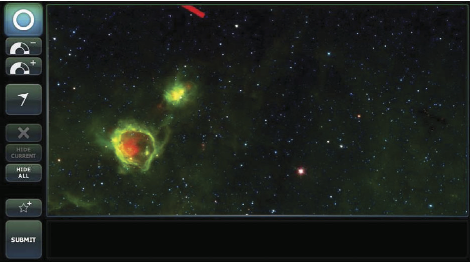
\includegraphics[width=\linewidth]{figs/SimpsonEtal2012_interface.png}
  \end{minipage}\hfill
  \begin{minipage}{0.51\linewidth}
    \centering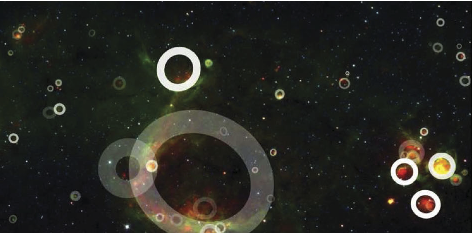
\includegraphics[width=\linewidth]{figs/SimpsonEtal2012_bubbles.png}
  \end{minipage}\hfill
\end{minipage}
\medskip

\begin{minipage}{\linewidth}
  \begin{minipage}{0.48\linewidth}
    \centering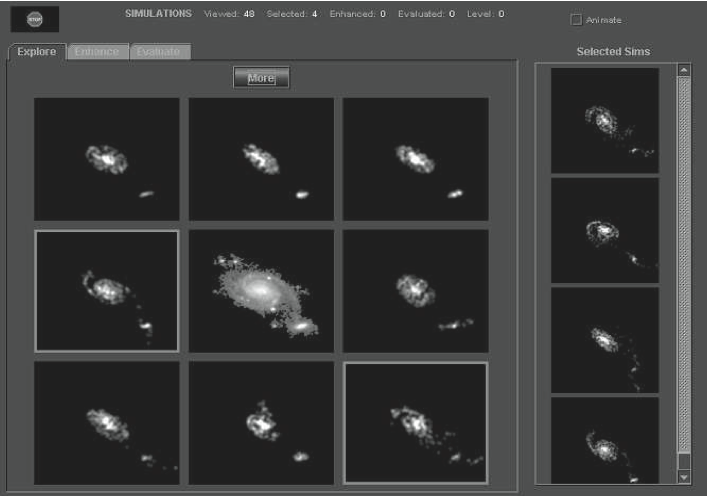
\includegraphics[width=\linewidth]{figs/HolincheckEtal2010_comparing.png}
  \end{minipage}\hfill
  \begin{minipage}{0.48\linewidth}
    \centering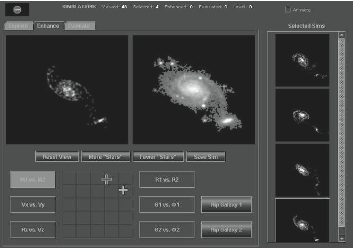
\includegraphics[width=\linewidth]{figs/HolincheckEtal2010_enhancing.png}
  \end{minipage}\hfill
\end{minipage}
\caption{Examples of image modeling in web-based citizen science projects. Top
row: star formation ``bubble'' identification and interpretation in Spitzer
images in the Milky Way Project, with the annotation interface shown on the
left, and some example (selected, averaged) bubbles on the right. Images from
\citet{SimpsonEtal2012}. Bottom row: matching N-body simulated merging
galaxies to SDSS images in the Galaxy Zoo Mergers project (left), and
exploring parameter space two parameters at a time to refine the models
(right). Screenshots from \citet{HolincheckEtal2010}.}
\label{fig:modeling}
\end{figure}
%%%%%%%%%%%%%%%%%%%


The above examples involved modeling infrastructure provided by either the
project's developers or science teams. There have also been cases where
citizens have carried out modeling analyses using their own tools, or writing
their own software. For example, in the PlanetHunters project, a small group
[?] of volunteers downloaded full Kepler lightcurve datasets for the best [?]
community-selected candidates, and fitted transit lightcurves to them using
[?]. [Chris: can you please confirm and extend this?]

Another very interesting case is the Pascal and Kaggle analysis challenges
organised by the professional cosmology community.  The measurement of weak
gravitational lensing by large scale structure (``cosmic shear'') relies on
the measurement of the shapes of distant, faint galaxies with extreme
accuracy. The STEP \citep{HeymansEtal2006,MasseyEtal2007} and GREAT
\citep{BridleEtal2010,KitchingEtal2012,KitchingEtal2013a} blind galaxy shape
estimation challenges have had an enormous impact on the field, revealing
biases present in existing techniques, and providing a way for researchers
outside the world of professional cosmology to participate. In particular, the
GREAT08 challenge saw very successful entries (including the winner) from two
(out of a total of 11) teams of researchers from outside the field. 



A subsequent, somewhat simplified
challenge was hosted at the Kaggle website \citep{KitchingEtal2013b}.

Kaggle challenges: shape estimation, mass clump positioning. 
GREAT challenge, compare and contrast.


% \BLOG{??}{Phil}{What's the most difficult thing a crowd can do?}
% \item Neptune encounter (what is this?!)

% - - - - - - - - - - - - - - - - - - - - - - - - - - - - - - - - - - - - - - - 

\subsection{Data Modeling in Other Fields (\textbf{Phil}, Chris, 2 pages)}
\label{sec:model:astro}

Case studies:
\begin{itemize}
\item Protein folding with Fold.it. Gamification as a technique.
\item Other examples: look around SciStarter. 
\end{itemize}

% \BLOG{??}{Phil}{Who's really doing all the work?}


% ------------------------------------------------------------------------------

\section{Data Exploration: Citizen Enquiry (3 pages)}
\label{sec:explore}

The previous sections have focused on specific, and isolated, activities in
which citizens have participated. In most cases, the community's involvement has
been a {\it contribution} to a scientific investigation, while not being
involved in the design of the investigation. The most important part of any
scientific investigation is the question at the heart of it: what is it we are
trying to find out about the world? In this section we look at some cases where
the process of enquiry, the science, has been instigated or led by citizens.  In
principle, this is an area of great potential. Professional scientists can find
it very difficult to step back from the technical details of their work, and see
the bigger picture; in contrast, outsiders only see the big picture, and  so we
might expect them to ask some unusual, surprising and searching questions. 


% - - - - - - - - - - - - - - - - - - - - - - - - - - - - - - - - - - - - - - - 

\subsection{Individuals in action (Phil to edit, 1 page)}
\label{sec:explore:individuals}

The constraints of funding proposals and management of research groups can
often mean that professional scientists focus very narrowly on particular
topics of research, using a particular technique for which they become known. 
Steering away from this course implies taking risks with time management, and
allocation of resources to an ultimately fruitless research area can be
detrimental to careers.  Citizen scientists are largely free of these
managerial and budgetary constraints, and are able to devote their attentions
to whatever topics interest them.  We propose that the creativity of citizen
scientists, and the freedom to ask questions and direct scientific enquiry, is
nurtured by the creation of communities.  These can be online communities,
with individuals contributing ideas via discussion groups and challenging one
another; or they can be ready-made communities, such as school classes and
family groups. 

Online forums arguably provide the most direct connection between citizens and
professional scientists, and have already been discussed in this review. 
Examples of individual successes include the ?Saturn Storm Watch? connecting
Cassini?s observations of lightning emissions with active amateur observations
of convective cloud structures within the giant planet atmosphere; and the
tracking of the vertices of Saturn?s bizarre north polar hexagon
\citep{88godfrey}, a 6-sided planet encircling wave that has persisted for at
least 30 years but that has only recently been observed by amateur
astronomers.  In the first case, citizen scientists wished to identify the
source of Saturn?s radio emissions.  In the latter case, the long-term
evolution of the hexagon vertices is being used to understand what sort of
wave this is, and to identify its origins.

Astronomy as an educational tool has been used to encourage a whole new
generation of citizen astronomers, and the aid of teachers in guiding and
encouraging the enquiries of school children is essential for the teaching of
the scientific method.  The Faulkes telescope is an excellent example of
citizen-led enquiry ? both student-devised and teacher-led investigations can
be performed at the network of robotic observatories in Hawaii and Australia,
allowing students to develop scientific questions using their own data and
collaboration with other students around the world.  A selection of some of
these projects can be found here: 
http://www.faulkes-telescope.com/showcases/schools.  Other observatories
around the world have telescopes devoted to citizen enquiry ? the Pic-du-Midi
observatory\footnote{http://www.obs-mip.fr/pic-du-midi} in the French Pyrenees
has a 0.6-m telescope devoted to amateur observers.   For example, in 2013 M.
Delacroix used the 1-m observatory to image details on Uranus and
Neptune\footnote{http://www.cloudynights.com/ubbthreads/showflat.php/Cat/0/Number/5955129/page/0/view/collapsed/sb/5/o/all/fpart/1/vc/1}.

Case studies:
\begin{itemize}
\item Teacher-led science: Blackawton Bees. 
\item Families as research groups: Monster eyes. % http://blogs.discovermagazine.com/notrocketscience/2012/10/30/12-year-old-uses-dungeons-and-dragons-to-help-scientist-dad-with-his-research/
\end{itemize}


% - - - - - - - - - - - - - - - - - - - - - - - - - - - - - - - - - - - - - - - 

\subsection{Facilitated research groups (\textbf{Chris}, Phil, 2 pages)}
\label{sec:explore:groups}

Case studies:
\begin{itemize}
\item Galaxy Zoo forum. Voorwerp, Green Peas. Lens thread: search and model.
\item Planet Hunters' investigations
\item Quench.
\item Deep sky obs (variable nebulae etc). Amateur asteroid observations and follow-up.
\end{itemize}

% ------------------------------------------------------------------------------

\section{Understanding the Citizens (2 pages)}
\label{sec:crowd}

Having surveyed some of the activities involving citizen scientists, we can
now consider some questions about this community itself. Who participates in
citizen science, and what motivates them?


% - - - - - - - - - - - - - - - - - - - - - - - - - - - - - - - - - - - - - - - 

\subsection{Demographics (Chris to finish, 1/2 page)}
\label{sec:crowd:demographics}

Who is participating in citizen astronomy? We might expect the demographics to
vary with activity, and with the level of commitment required. We have some
understanding of at least the former division from two studies that were
carried out approximately simultaneously, one of the community  participating
in Galaxy Zoo, and another of the  American Association of Variable Star
Observers (AAVSO).  \citet{Rad++13} surveyed the Galaxy Zoo volunteer
community to investigate their motivations (\Sref{sec:crowd:motivation}
below), via a voluntary online questionnaire. The 11,000 self-selected Galaxy
Zoo users identified as 80\% male, with both genders having an approximately
uniform distribution in age between their mid-twenties and late fifties. The
authors point out that this is close to the US internet user age distribution,
except for slight but significant excesses in numbers of post-50s males,
post-retirement people of both genders, and a deficit in males under 30. The
survey respondents  also tended to be more highly educated than average US
internet users, with most holding at least an undergraduate degree, and around
a quarter having a masters or doctorate. 

These findings can be compared with a survey of the members of AAVSO:
\citet{P+P2012} received over 600 responses  (corresponding to about a quarter
of the community of observers and society members). The education levels of
the AAVSO repondents matches the Galaxy Zoo community very closely; the AAVSO
age distribution is more peaked (in the mid fifties), with a similar post-60
decline but also a marked absence of younger people. The online nature of the
Galaxy Zoo project seems to have increased the participation of younger (pre
middle-age) people. Likewise, the Galaxy Zoo gender bias, while itself
extreme, is less so than at AAVSO, where some 92\% of survey respondents were
male. One additional piece of information provided by the AAVSO survey is the
profession of the variable star observers: most (nearly 60\%) of the survey
respondents were found to be working in science, computer science, engineering
and education.

The Galaxy Zoo and AAVSO communities differ by more than just the nature of
their activity. The smaller AAVSO community is arguably more engaged in its
research, in the sense that a larger fraction of its membership is active in
taking observations and contributing to analyses. It would be very interesting
to know how citizen scientist motivation varied with the level of
participation: dividing the Galaxy Zoo community into volunteers that
contribute to the  forum and those who don't could be interesting; perhaps
more so would be to repeat the analysis of \citeauthor{Rad++2013} over a wide
range of projects, and look for trends there. The emergent picture thus far,
however, is of a well-educated (and often scientifically trained)  but
male-dominated citizen science community, whose female and younger membership
is likely to have been, at least in part, enabled via projects being hosted
online. Continuing to lower the barriers to entry for currently
under-represented demographic groups would seem both important, and within
reach.


% - - - - - - - - - - - - - - - - - - - - - - - - - - - - - - - - - - - - - - - 

\subsection{Motivation (Chris to finish, 1 page)}
\label{sec:crowd:motivation}

What motivates citizen scientists? The two demographic studies referred to
above also covered this question; it was the primary motivation for
\citeauthor{Rad++2013}. Having previously identified 12 categories of
motivation in an earlier pilot study \citep{Rad++2010}, \citeauthor{Rad++2013}
asked the 170,000 volunteers at the time to comment on how motivated they were
by each of these categories, and which was their primary motivation. The 6\%
who responded gave consistent answers to around 900 forum users who responded
in a separate appeal, allowing us to draw conclusions about this presumably
more engaged sub-population. A desire to {\it contribute} to science was found
to be the dominant primary motivation, being selected by 40\% of respondents.
{\it Astronomy}, {\it science}, {\it vastness}, {\it beauty} and 
{\it discovery} were all motivation categories that were found to very
important to the volunteers, while {\it fun}, {\it learning} and {\it
community} were less important. 

The AAVSO demographic survey \citep{P+P2012} found similar results: over a
third of variable star observers cited involvement in science and research as
their primary source of motivation. However, a similar number gave an interest
in variable stars as theirs, perhaps reflecting a stronger focus on the
science questions involved than is present in the Galaxy Zoo community. Both
groups of citizen scientists are clearly quite serious in their reasons for
taking part: their motivations are actually very close to those of
professional scientists, as many readers of this review will recognize.

These surveys reveal a community of people many of whom may have left  
academic science behind as soon as they finished their  education, but who
still maintained a passion for astronomy and the  boundaries of knowledge. 
Their thirst for knew information, and the  desire to be part of the 
scientific process drives them to actively observe the  night sky or to
participate in analysis of large datasets.  

For many people involved in citizen science, being part of a community, 
albeit a distributed one, that brings great enjoyment and satisfaction.  With
the connectivity of the internet, there is a social  aspect of citizen science
that unites people with shared interests.   These pastimes and hobbies are
often far removed from someone's ``normal''  life. However, {\it community}
was not found to be a strong motivator for the Galaxy Zoo volunteers -- but it
is nevertheless very important for the Galaxy Zoo forum users. More recent
Zooniverse projects have sought to widen participation in community
discussion, hypothesizing not that it will motivate people better, but because
it will help them make better contributions. Citizen scientists, like
professional scientists, are primarily motivated by getting science done.


% ------------------------------------------------------------------------------

\section{Summary: Characteristics of Successful Citizen Science (1 page)}
\label{sec:summary}

To emerge.

Uncompromising stance on value of citizen contributions: focus on tasks that
cannot be done by machines or professionals.

Low barrier to entry, easy to make a contribution.

Emphasis on science that volunteeris to be part of. 

Good communication between professionals and citizens.

High level of respect for volunteers: think of citizens as collaborators,
research assistants.

The need to understand black box systems -- especially if the box is full of
people. But: people must be treated as ends in themselves. 

% ------------------------------------------------------------------------------

\section{Ideas for the future (possibly absorbed into sections above?) (4 pages)}
\label{sec:future}

Preamble.

\phil{Should these parts be folded into the sections above? This might make for
an easier to read article.}

% - - - - - - - - - - - - - - - - - - - - - - - - - - - - - - - - - - - - - - - 
% 
% \subsection{Brief Notes on Methodology}
% \label{sec:future:method}
% 
% Crowd-sourced idea generation.  Invited contributions from everywhere. 
% Publicise to dotastronomy, facebook astronomers, twitterverse, wider still.
% Track and analyze.
% 
% Organise and critically review submissions, and submitters. Selection bias.
% Who is motivated? Who self-selected? 
% 
% - - - - - - - - - - - - - - - - - - - - - - - - - - - - - - - - - - - - - - - 

\subsection{Observations and Instrumentation in the future}
\label{sec:future:obs}

Robotic or automated telescopes to feed data to amateur processors/users for
immediate analysis.  Long term baselines with the same 
instrument/calibration.

Global telescope networks for continuous monitoring.
Distributed stations and networks for stellar occultations by TNOs and KBOs. 
Mobile observing stations and international coordination?

Video monitoring for meteors from multiple interlinked stations for 3D
trajectory reconstruction.

Amateur observing follows professional:
\begin{itemize}
\item Deeper field for amateur observations of Uranus and Neptune, particularly
near-IR.
\item Visible-light and near-IR spectroscopy; long-term datasets, serious
photometry.  Calibration, calibration, calibration...
\item Advanced technologies such as AO for image stabilisation?
\end{itemize}

Adoption of uniform standards for amateur imaging to be provided to online
databases (already underway with PVOL).


% - - - - - - - - - - - - - - - - - - - - - - - - - - - - - - - - - - - - - - - 

\subsection{Classification in the future}
\label{sec:future:class}

Live data: task assignment. 

Human-computer partnerships. Replacing citizens, see SN Zoo.

% Citizen access to crowd results?

% - - - - - - - - - - - - - - - - - - - - - - - - - - - - - - - - - - - - - - - 

\subsection{Data modelling in the future}
\label{sec:future:models}

Easily installed apps or browser-based tools enable outsourcing of data
modelling. Operation of code, development of code. Crowd-sourcing of current
detailed analyses.


% - - - - - - - - - - - - - - - - - - - - - - - - - - - - - - - - - - - - - - - 

\subsection{Scientific enquiry in the future}
\label{sec:future:enquiry}

Huge public databases from wide field surveys: LSST, Euclid, SKA. User
interfaces designed for anyone, with social networking enabled. 

Provide publishing support, see Letters.


% ------------------------------------------------------------------------------

\section{The Limits of Citizen Science (3 pages)}
\label{sec:limits}

We have argued that a critical part of `citizen science' lies in the ability of
the amateur to make an authentic contribution to science. Earlier in this part
of the review, we looked forward to a richer future for such interaction, but in
this section we consider the potential limits and checks on citizen science. 

% - - - - - - - - - - - - - - - - - - - - - - - - - - - - - - - - - - - - - - - 

\subsection{Data limits data rates: some worked examples}
\label{sec:limits:data}

Problems presented by data volume, and data rates. 
Case studies: Large samples of lenses?  Transients with SKA? 


% - - - - - - - - - - - - - - - - - - - - - - - - - - - - - - - - - - - - - - - 

\subsection{Limits from complexity}
\label{sec:limits:complexity}

Difficult analyses. Microtasking only suitable for certain parts of the process?


% - - - - - - - - - - - - - - - - - - - - - - - - - - - - - - - - - - - - - - - 

\subsection{Limits to collaboration}
\label{sec:limits:collab}

Collaboration between professional and citizen astronomers. Does it scale?
Communication issues: forum, letters. Contrast supervisor to student, with
scientist to crowd. Prospects for large collaborations? Collaborations between
citizens, eventually linked to professionals?

Relationships between citizens and professionals. Mostly one-way? Examples of
two-way interactions: zoo forum, solar system monitoring, spacecraft support.


% - - - - - - - - - - - - - - - - - - - - - - - - - - - - - - - - - - - - - - - 

\subsection{Limits to access}
\label{sec:limits:access}

Connections between citizen science and open data, and open publishing. 
Citizens reading papers: accessibility, potential barriers. 

International CS. Language barriers, cultural issues. 

Fast and reliable access  to the internet is
a pre-requisite for participation, and active  observation typically requires
financial investment in equipment,  biasing the demographics to the developed
world.  An alternative is  participation in educational projects such as the
Faulkes telescope,  providing access to world-leading equipment for
educational purposes.

% ------------------------------------------------------------------------------

\section{Concluding Remarks (1 page)}
\label{sec:conclusions}

Does astronomy have any sort of special place in citizen science?

Breaking down of boundaries. Professionals are citizens when outside their own
field. Citizens turning professional.

% ------------------------------------------------------------------------------

\section*{Acknowledgments}

% We are most grateful to everyone who took the time to deposit their two cents
% in the comments section of the \stellarpops blog, and in particular the
% following contributors whose ideas helped shape \Sref{sec:future} but were not
% cited by name in the text: XXX, YYY, ZZZ. 

PJM thanks the Royal Society for financial support in the form of a university
research fellowship. 
%
CJL is grateful...
%
LDF acknowledges...
% 
This work was supported by...

% ------------------------------------------------------------------------------
% Here is a test sentence, with a test citation \citep{Lin++08}.

\section{Literature Cited}

% ARAA style:
\bibliographystyle{Astronomy}

% Use bibtex:
\bibliography{references}

% ------------------------------------------------------------------------------

\end{document}

% ==============================================================================
